\Exhibit{GitHubStars}{%
    Справочная страница GitHub о звёздах репозиториев%
}

Этот скриншот показывает, что количество звёзд репозитория -- это метрика
популярности проекта.

\ParagraphQuote{%
    Звёзды, которые вы ставите, позволяют легче найти репозиторий или тему позже\dots
    Звёзды также означают признательность автору за его работу.
    Многие рейтинги репозиториев на GitHub основаны на количестве звёзд.
    Кроме того, Explore GitHub показывает популярные репозитории по количеству звёзд.%
}

\begin{center}
    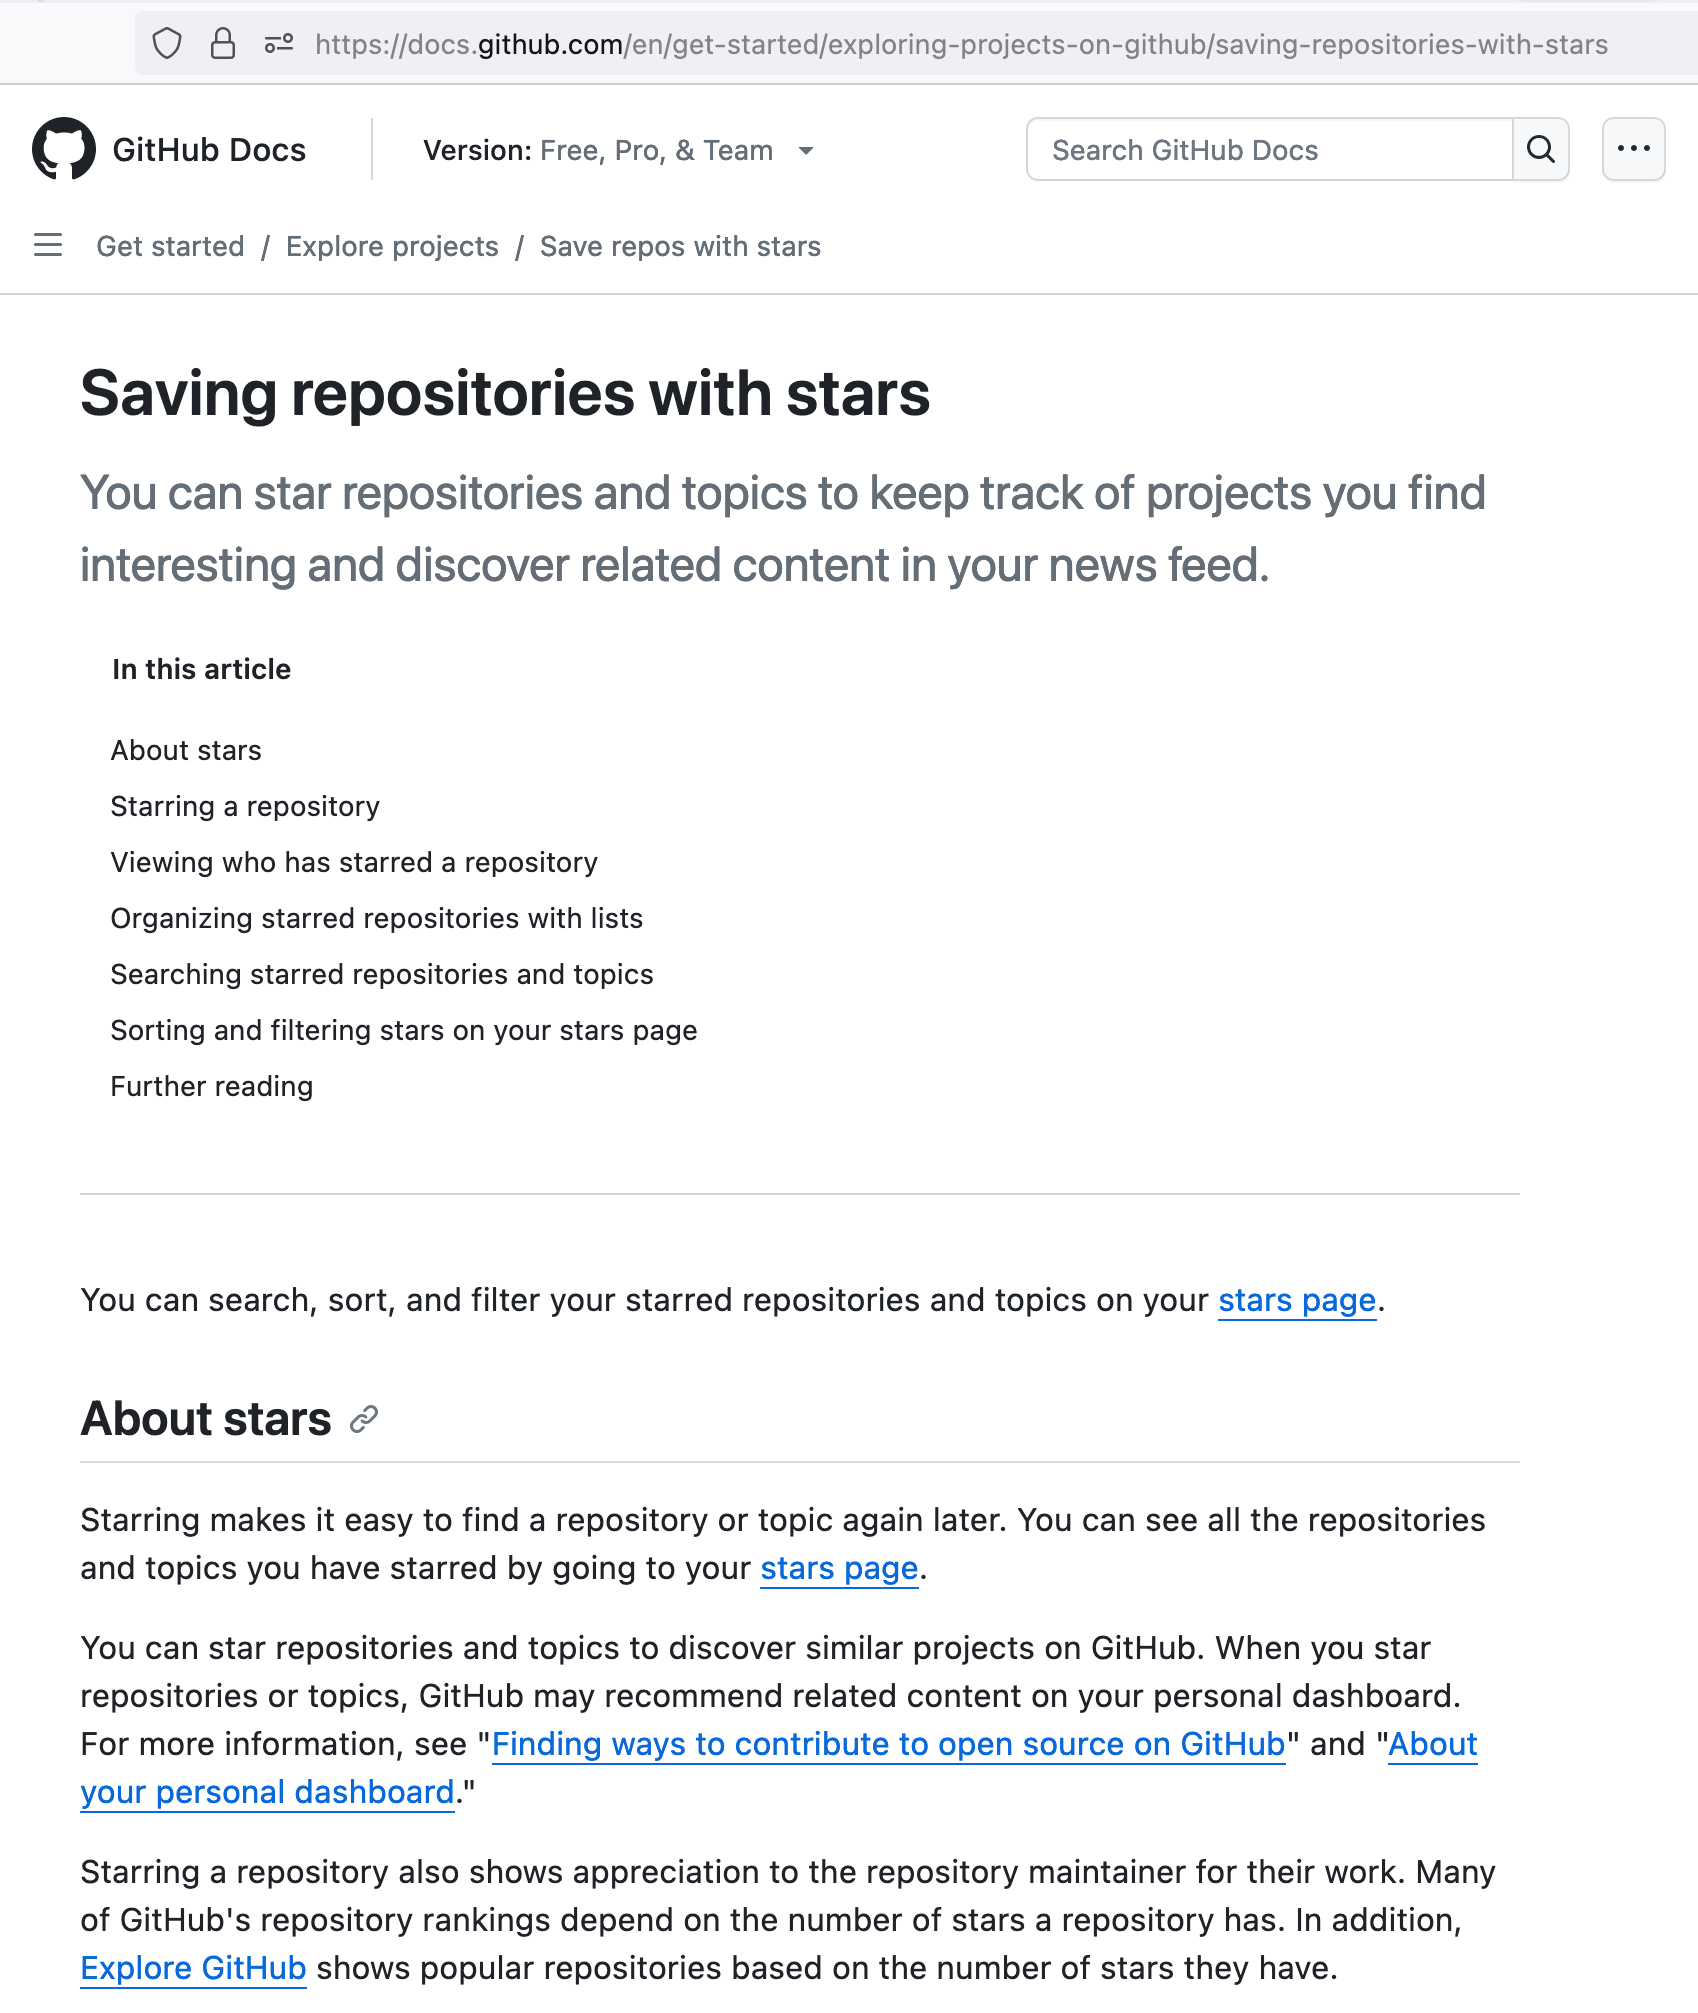
\includegraphics[width=30em]{github-stars}
\end{center}

\pagebreak
